%% appendix_features.tex — Feature Engineering: Scientific Basis and Implementation
%% Extracted from main.tex
\chapter{Feature Engineering: Scientific Basis and \\ Implementation}
\label{app:features}

The eight habitability-proxy features are extracted from the Cassini data
sources described in Appendix~\ref{app:notation}.  Each subsection gives the
scientific basis, prior mean justification, implementation procedure, and
missing-data backfill strategy.  Features derived from SAR backscatter ($f_1$, $f_3$, $f_5$, $f_7$, $f_8$) are affected by the $\sim$35\% areal coverage of the Cassini RADAR SAR imaging mode; in unmapped regions, the pipeline assigns physically motivated floor values rather than interpolated estimates.  No published method exists for interpolating SAR backscatter intensity on Titan: unlike topography, which varies smoothly and can be splined from sparse profiles \citep{Lorenz2013,Corlies2017Titan}, backscatter depends on local roughness, composition, and viewing geometry and lacks the spatial autocorrelation needed for meaningful gap-filling.

Figure~\ref{fig:feature_panel} shows all eight feature maps at the present
epoch, illustrating their distinct spatial patterns.  Figure~\ref{fig:epoch_timeline}
shows how the relative activity of each feature is modulated across geological
time.

All features are normalised to the range $[0, 1]$ using a robust
percentile-clipping approach:
\begin{equation}
  \hat{f}_i = \mathrm{clip}\!\left(
    \frac{f_i - f_{i,\text{p2}}}{f_{i,\text{p98}} - f_{i,\text{p2}}},
    \; 0, \; 1
  \right)
  \label{eq:normalise_app}
\end{equation}
where $f_{i,\text{p2}}$ and $f_{i,\text{p98}}$ are the 2nd and 98th
percentiles of finite values in the global layer, mapping the central 96\%
of the observed dynamic range onto $[0, 1]$ whilst preventing extreme outliers
from compressing the scale.  Where a feature is unavailable at a particular
pixel (due to data gaps), the value is set to NaN and handled through the
Bayesian missing-data imputation procedure described in Section~\ref{sec:nan}.

\begin{figure}[H]
  \centering
  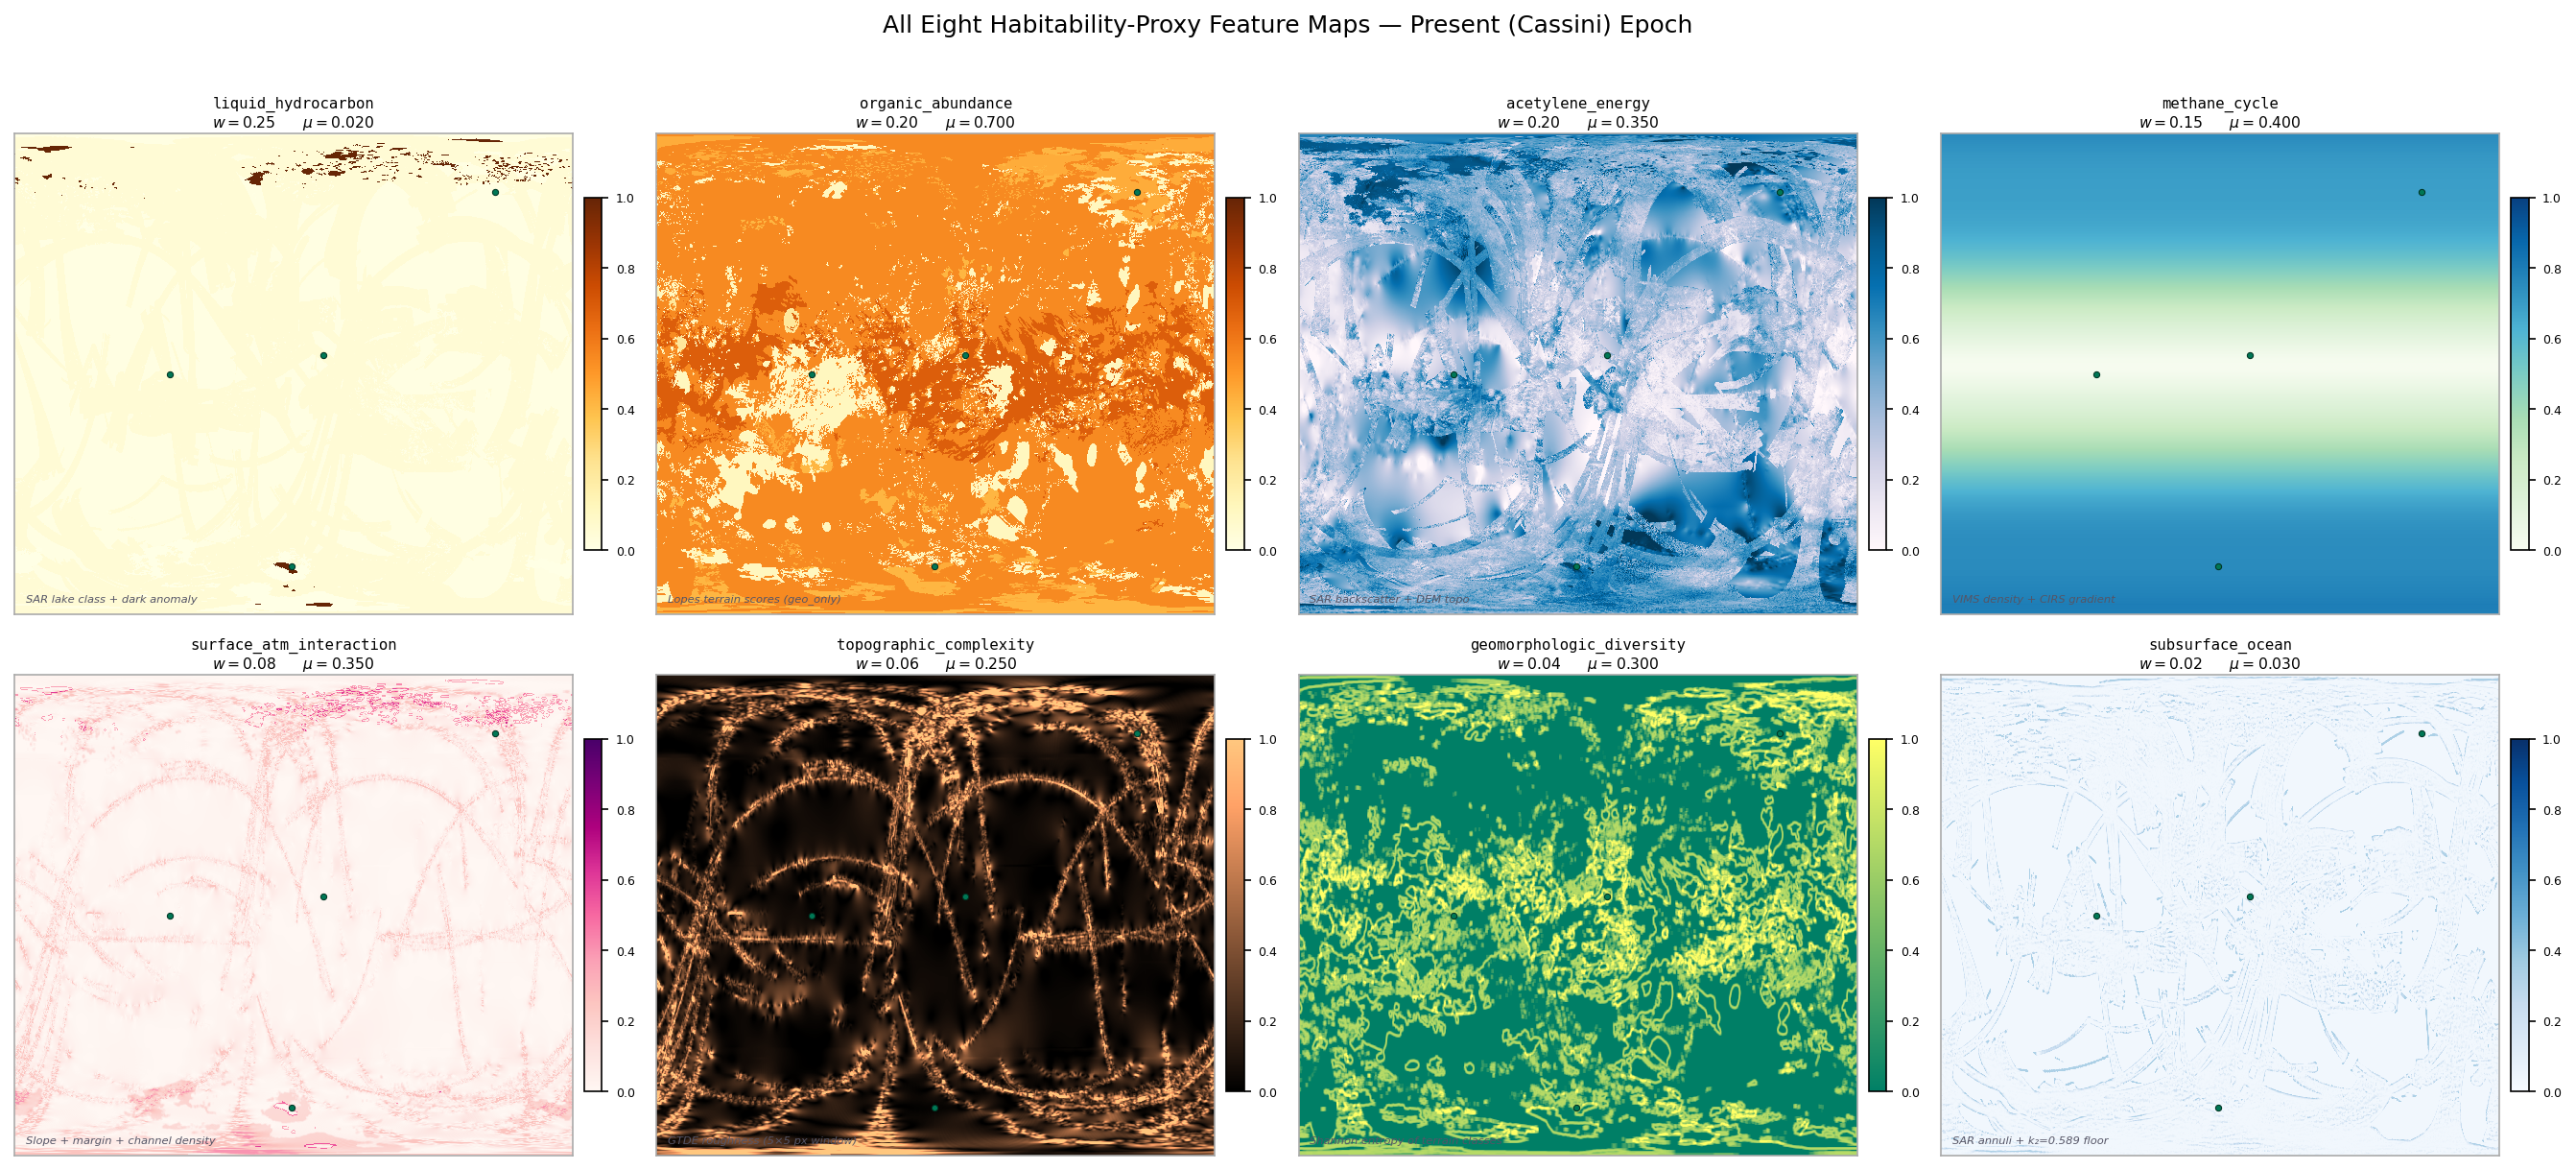
\includegraphics[width=\textwidth]{images/feature_panel_present.png}
  \caption{All eight habitability-proxy feature maps at the present (Cassini)
    epoch, each normalised to $[0,1]$.  The panels illustrate the distinct
    spatial patterns contributed by each feature: the polar concentration of
    liquid hydrocarbon ($f_1$), the near-global organic abundance ($f_2$),
    the topographically-modulated chemical energy proxy ($f_3$), and the
    latitude-dependent methane cycle signal ($f_4$), amongst others.  The
    combined posterior is derived from all eight simultaneously via the
    Bayesian update described in Section~\ref{sec:bayes}.  Prior weight $w_i$
    and prior mean $\mu_i$ are shown for each panel.  Blank (white) regions
    indicate pixels where the feature data is unavailable due to Cassini
    coverage gaps (primarily in SAR-dependent features $f_1$, $f_3$, $f_5$,
    $f_7$, $f_8$); these pixels are imputed with the feature prior mean
    $\mu_i$ during the Bayesian update (Section~\ref{sec:nan}), contributing
    no evidence rather than incorrect evidence.  The vertical discontinuity
    visible in $f_3$ at 180\textdegree{}W is an assembly seam in the USGS
    SAR mosaic (\texttt{clon180} product), where flyby swaths from opposite
    hemispheres were stitched at the mosaic's central meridian; this artefact
    propagates through the SAR backscatter component of the acetylene energy
    proxy but is attenuated in the posterior by the 20\% weight of $f_3$.}
  \label{fig:feature_panel}
\end{figure}

\begin{figure}[H]
  \centering
  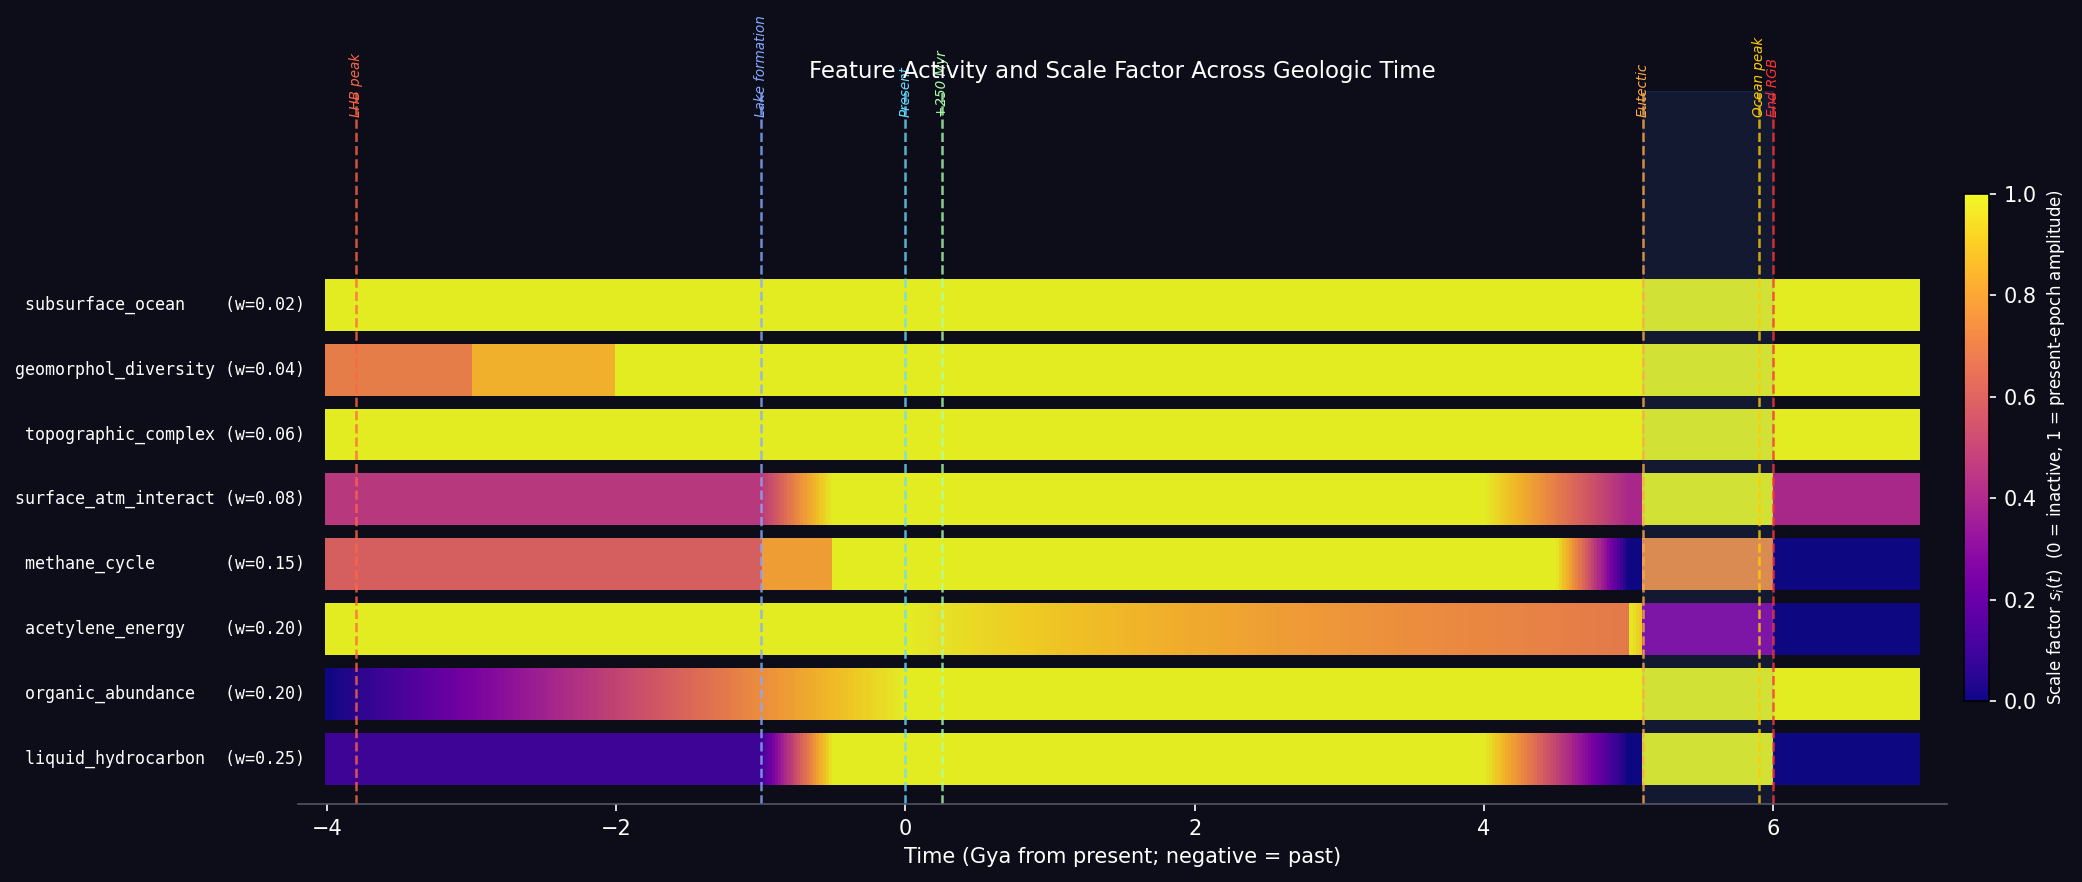
\includegraphics[width=\textwidth]{images/epoch_feature_timeline.png}
  \caption{Scale factor (relative activity) for each feature as a function
    of geological time from $-4.0\gya$ to $+7.0\gya$.  Colour intensity
    encodes the scale applied to each feature's prior mean at that epoch:
    bright yellow indicates full present-epoch amplitude; dark blue indicates
    near-zero activity.  Key events (LHB peak, lake-formation onset, present
    epoch, solar warming ramp, eutectic crossing, ocean peak) are marked with
    vertical dashed lines.  The impact-melt proxy and cryovolcanic flux
    features are active only in pre-lake epochs and are shown in the lower
    two rows.}
  \label{fig:epoch_timeline}
\end{figure}

\section[Feature 1: Liquid Hydrocarbon Availability
  ($w_1 = 0.25, \mu_1 = 0.02$)]{Feature 1: Liquid Hydrocarbon Availability \\
  ($\boldsymbol{w_1 = 0.25, \mu_1 = 0.02}$)}
\label{sec:feat_lhc}

\paragraph{Scientific basis.}
Liquid methane and ethane are the proposed non-aqueous biochemical solvents
for any life operating on \titan{}'s present-day surface \citep{McKaySmith2005,
McKay2016}.  At the ambient surface temperature of $\sim$94\,K, water is
structurally as rigid as rock and cannot support molecular diffusion processes
fundamental to metabolism.  Liquid methane and ethane are, however, stable
at 94\,K and 1.47\,bar, as confirmed by the permanent north polar seas.
\citet{Benner2004} proposed that non-polar solvents can in principle support
biochemistry through different but self-consistent molecular architectures, and
\citet{Stevenson2015} demonstrated through molecular dynamics simulations that
acrylonitrile molecules present in \titan{}'s atmosphere can form stable
vesicle membranes in liquid methane.  The presence of persistent liquid
hydrocarbon is therefore treated as the single most important habitability
prerequisite for surface life at the present epoch, and accordingly receives
the highest prior weight ($w_1 = 0.25$).

\paragraph{Prior mean.}
The north polar seas cover approximately 1.5--2\% of \titan{}'s surface
\citep{Hayes2008}, giving a prior mean of $\mu_1 = 0.02$.  Despite the high
weight, the low prior mean means that most pixels contribute negligibly through
this feature; its habitability impact is strongly localised to the polar
regions.

\paragraph{Implementation.}
The primary source is the Lopes et al.\ (2019) lake polygon class (terrain
class 7), rasterised to the canonical grid as a binary lake mask.  A secondary
contribution comes from SAR backscatter dark anomalies not otherwise attributed
to organic material.  Confirmed empty lake basins from the Birch et al.\ (2017)
analysis are explicitly assigned $f_1 = 0$ to reflect the absence of
present-day liquid even within geomorphologically defined basins.  In the
absence of SAR coverage, ISS 938\,nm albedo imagery provides a proxy, with
smooth, low-albedo regions consistent with liquid surfaces elevated towards
higher feature values.

\paragraph{Backfill.}
In regions lacking both SAR and ISS coverage, the feature is assigned NaN and
imputed at the prior mean during inference.

\section[Feature 2: Organic Abundance
  ($w_2 = 0.20$, $\mu_2 = 0.70$)]{Feature 2: Organic Abundance
  ($\boldsymbol{w_2 = 0.20, \mu_2 = 0.70}$)}
\label{sec:feat_organic}

\paragraph{Scientific basis.}
Tholins (the complex refractory macromolecular organic compounds produced
continuously by ultraviolet photolysis of the \ce{N2}/\ce{CH4} mixture in the
upper atmosphere) are the dominant surface material across most of \titan{}.
Laboratory hydrolysis of
tholins in liquid water at biologically relevant temperatures (273--373\,K)
produces amino acids, nucleobase analogues, and sugar-like polyols at yields
of $\sim$0.1\% by mass \citep{Neish2010}, directly confirming that tholins
can serve as a chemical feedstock for prebiotic synthesis when liquid water
is available: either from impact melts at past epochs or from the red-giant
ocean in the far future.  \citet{MeyerDombard2025} characterise the tholin
layer as the primary chemical substrate for any surface habitability scenario
on \titan{}.  The feature weight ($w_2 = 0.20$) is second only to liquid
hydrocarbon, reflecting this central role.

\paragraph{Prior mean.}
The revised prior mean of $\mu_2 = 0.70$ (updated from 0.60 in earlier
pipeline versions) reflects updated spectral characterisation from
\citet{Malaska2025} and \citet{Cable2012}, indicating that approximately 82\%
of the SAR-classified surface by area falls into organic-rich terrain classes
(dune: 17\%, plains: 65\%).  The organic abundance feature consequently makes
the largest single contribution to the global prior mean
($w_2\mu_2 = 0.140$).

\paragraph{Implementation and the blended VIMS mosaic.}
The primary spectral data source is the VIMS+ISS 1.59/1.27\,\textmu{}m
band-ratio mosaic from \citet{Seignovert2019CaltechDATA}, but this covers
only the 0--180\textdegree{}W hemisphere ($\sim$50\% of the globe).  Extensive
testing of direct blending between the VIMS band ratios and geomorphological
class scores in the 180--360\textdegree{}W hemisphere produced a visible seam
artefact at the 180\textdegree{}W boundary: the absolute calibration of the
VIMS spectral ratio differs systematically from the terrain-class score at
the coverage boundary, producing a step change of $\sim$0.13 in median organic
abundance clearly visible in rendered maps.  The analysis resolves this with a global offset correction:
the median VIMS value in the overlap region between VIMS and terrain-class
coverage is aligned to the corresponding median terrain-class score,
eliminating the boundary discontinuity while preserving per-pixel spectral
variation within the VIMS-covered hemisphere.  In the remaining hemisphere,
terrain-class scores from Table~\ref{tab:geo_scores}
(Appendix~\ref{app:geo_scores}) are used directly.  This blended approach
retains the spectral resolution of the VIMS data (standard deviation 0.27)
at polar lake sites where per-pixel organic variation is scientifically
significant, while maintaining seamless global coverage.\footnote{The
Seignovert VIMS+ISS mosaic uses IAU east-positive longitude
(\citealt{Seignovert2019CaltechDATA}; confirmed by the 2019 LPSC abstract
referencing landmarks at east-positive coordinates).  The pipeline canonical
grid uses west-positive longitude.  Conversion requires a horizontal flip
of the pixel array (not a 180\textdegree{} roll), because the two conventions
differ in column ordering direction, not origin.  Alignment was validated by
three tests: (i)~Kraken Mare (310\textdegree{}W) shows VIMS spectral texture
(local $\sigma > 0.02$); (ii)~no step change at the 180\textdegree{}W
hemisphere boundary ($|\Delta P(H)| < 0.02$ at all latitude bands); and
(iii)~the rendered global maps show smooth spatial gradients consistent
with the Cassini-era geomorphological observations.}

\paragraph{Backfill.}
The Lopes (2019) terrain classification covers $\sim$90\% of the SAR-imaged
surface ($\sim$67\% of the globe).  In regions outside SAR coverage, terrain
class is estimated from ISS albedo units with reduced specificity.

\section[Feature 3: Chemical Energy Availability
  ($w_3 = 0.20$, $\mu_3 = 0.35$)]{Feature 3: Chemical Energy Availability \\
  ($\boldsymbol{w_3 = 0.20, \mu_3 = 0.35}$)}
\label{sec:feat_energy}

\paragraph{Scientific basis.}
Life requires a sustained source of chemical free energy to drive metabolic
reactions against thermodynamic equilibrium.  On \titan{}'s surface, the
primary candidate is acetylenotrophy ($\ce{C2H2 + 3H2 -> 2CH4}$, $\Delta G = -334$\,kJ\,mol$^{-1}$; where $\Delta G$ is the Gibbs Free Energy
change of the reaction, a negative value indicating spontaneous energy release)
available from acetylene--hydrogen combination \citep{McKaySmith2005}.  \citet{Yanez2024} recalculated the
available energy under updated thermochemical conditions at \titan{}'s surface
as 69--78\,kJ\,mol$^{-1}$\,C, well above the minimum for terrestrial
methanogens.  Acetylene is produced continuously by UV photolysis of methane
and sediments to the surface where it has been directly detected by GCMS
\citep{Niemann2005}.  The chemical energy feature is therefore a proxy for
the co-availability of acetylene and hydrogen at the surface.

\paragraph{Implementation.}
Since the acetylene surface abundance cannot be directly mapped by any Cassini
instrument, it is approximated through two components.  SAR backscatter
(weight 70\% where coverage exists): SAR-dark surfaces characteristic of
organic-rich terrain represent regions where acetylene is most likely to
accumulate without competing abiotic reactions consuming it rapidly.
Topographic inversion (weight 30\%): acetylene and other atmospheric
condensates preferentially accumulate in topographic lows through both
gravitational settling and fluvial transport; the normalised negative of
the GTDE elevation ($-z$) assigns high values to topographic lows.
In SAR-absent regions, the feature reverts to the pure topographic
inversion component.

\section[Feature 4: Methane Cycle Intensity
  ($w_4 = 0.15$, $\mu_4 = 0.40$)]{Feature 4: Methane Cycle Intensity \\
  ($\boldsymbol{w_4 = 0.15, \mu_4 = 0.40}$)}
\label{sec:feat_methane}

\paragraph{Scientific basis.}
The methane cycle is the dominant agent of chemical transport on \titan{}.
It delivers organic material from equatorial photochemical production regions
to the polar lake margins, maintains chemical gradients at shorelines, and
provides seasonal wet--dry cycling at lake edges that some prebiotic chemistry
scenarios identify as important for concentrating organic reactants and driving
condensation reactions \citep{Benner2004, MitchellLora2016}.  Regions
experiencing the most active methane cycling receive fresh organic inputs
most regularly and maintain the most dynamic chemical environments.

\paragraph{Implementation.}
The methane cycle intensity is a weighted composite of three independently
computed components:
\begin{enumerate}
  \item \textbf{VIMS observation density} (50\%): the number of VIMS
    spectral footprints per grid cell, smoothed with a 5-pixel Gaussian
    kernel.  Cassini's VIMS observation targeting was scientifically
    motivated, prioritising regions of active methane-cycle interest;
    higher coverage density therefore correlates with active methane
    cycling zones \citep{LeMouelic2019}.
  \item \textbf{Meridional temperature gradient} $|\partial T/\partial\phi|$
    (25\%): derived from the Jennings (2019) model (Eq.~\ref{eq:jennings}),
    evaluated at $Y = +1.39$ (year 2011.0, the approximate mission midpoint).
    Regions where the surface temperature gradient is steepest experience
    the strongest differential evaporation and precipitation, driving the
    most vigorous methane transport.
  \item \textbf{Latitude prior} (25\%): the function
    $\exp[-(\phi \pm 45\textdegree)^2/(25\textdegree)^2]$, following
    \citet{MitchellLora2016}'s general circulation modelling result that
    the mid-latitude regions host the primary methane cycle activity
    during the Cassini epoch.
\end{enumerate}

This feature has 100\% global coverage by construction and requires no
backfill.

\section[Feature 5: Surface--Atmosphere Interaction Intensity
  ($w_5 = 0.08$, $\mu_5 = 0.35$)]{Feature 5: Surface--Atmosphere Interaction Intensity \\
  ($\boldsymbol{w_5 = 0.08, \mu_5 = 0.35}$)}
\label{sec:feat_sai}

\paragraph{Scientific basis.}
The physical interface between surface and atmosphere is where gas-phase
photochemical products encounter potential liquid solvents and organic
substrates.  Lake margins and fluvial channel termini are the primary loci
of this exchange.  \citet{Hayes2016} describes the complex sedimentological
and chemical processes at hydrocarbon lake shorelines, including the
evaporation-driven concentration of dissolved organics and the seasonal
flooding and drying cycles that expose organic sediments to liquid contact.
\citet{Miller2021channels} documents that the fluvial channel network
terminates preferentially at polar lake margins, establishing these as zones
of maximum organic delivery and chemical gradient activity.

\paragraph{Implementation.}
A weighted sum of three spatial components:
\begin{equation}
  f_5 = 0.30\,\hat{s} + 0.40\,\hat{m} + 0.30\,\hat{c}
  \label{eq:feat5}
\end{equation}
where $\hat{s}$ is the normalised topographic slope $|\nabla z|$ from the
GTDE DEM (high slopes drive physical transport and mixing); $\hat{m}$ is a
binary lake-margin mask extended to $\sim$45\,km from the nearest confirmed
lake shore; and $\hat{c}$ is the Gaussian-smoothed ($\sigma = 3$ pixels)
channel density from the Miller et al.\ (2021) dataset, normalised at the
2nd--98th percentile range.  The lake-margin component receives the highest
within-feature weight (40\%) because shorelines concentrate all three relevant
processes: liquid contact, organic delivery, and thermal/chemical cycling.

\section[Feature 6: Topographic Complexity
  ($w_6 = 0.06$, $\mu_6 = 0.25$)]{Feature 6: Topographic Complexity \\
  ($\boldsymbol{w_6 = 0.06, \mu_6 = 0.25}$)}
\label{sec:feat_topo}

\paragraph{Scientific basis.}
Local topographic roughness at $\sim$20\,km scale correlates with the
dissected terrain types that most frequently expose water-ice-bearing crustal
material \citep{Lopes2019}.  On Earth, topographic heterogeneity at ecologically
relevant scales creates micro-environmental diversity (variations in
drainage, aspect, moisture, and chemical exposure) that underpins elevated
species richness at landscape boundaries.  On \titan{}, the analogous principle
is that varied topography produces diverse chemical micro-environments with
potentially richer reactive diversity.

\paragraph{Implementation.}
Local standard deviation of GTDE elevation computed in a $5\times5$ pixel
($\sim$22\,km) sliding window, normalised to $[0,1]$ at the 2nd--98th
percentile range.  South polar gaps in the primary GTDE are filled with the
Corlies et al.\ (2017) globally interpolated DEM prior to roughness computation.

\section[Feature 7: Geomorphological Diversity
  ($w_7 = 0.04$, $\mu_7 = 0.30$)]{Feature 7: Geomorphological Diversity \\
  ($\boldsymbol{w_7 = 0.04, \mu_7 = 0.30}$)}
\label{sec:feat_geodiv}

\paragraph{Scientific basis.}
Astrobiologically relevant chemistry is disproportionately likely to occur
at interfaces between geochemically distinct terrain types.  The reasoning
is thermodynamic: chemical gradients (differences in redox potential,
organic content, water-ice availability, or pH) drive reactions that would
not proceed in chemically uniform settings \citep{Shock2007}.  On \titan{},
the most important geochemical interfaces identified from Cassini data are:

\begin{enumerate}
  \item The \textbf{dune--plains boundary}, where organic-rich tholin-saturated
    dune sand is in direct lateral contact with the moderate-organic plains
    through which fluvial channels transport material towards the polar lakes.
    This interface concentrates the exchange between the primary
    photochemical organic source (dunes) and the active transport system
    (plains channels).

  \item The \textbf{crater ejecta interface}, where water-ice-rich crustal
    material excavated by impact is juxtaposed with adjacent organic-bearing
    terrain.  \citet{Neish2018} demonstrated experimentally that mixing
    water ice and tholins under liquid water conditions produces amino acids;
    the spatial co-occurrence of these two materials at crater ejecta
    boundaries is therefore a direct proxy for the relevant chemical
    reactivity.

  \item The \textbf{lake--plains/dune boundary}, where liquid hydrocarbon
    meets the organic substrate, enabling dissolution and transport of
    surface organics into the lake system.
\end{enumerate}

The Shannon entropy of terrain class distribution within a local window
quantifies the degree of terrain-type mixing at each pixel.  A pixel
surrounded by a single terrain class (entropy = 0) sits in a geochemically
homogeneous environment.  A pixel at the intersection of four terrain
classes (entropy approaching $H_\text{max}$) sits at a multi-way geochemical
interface.  This feature receives the second-lowest weight of the present-epoch set
($w_7 = 0.04$, above only subsurface-ocean proximity) because it is an indirect and geometrical proxy for chemical
gradients rather than a direct measurement.

\paragraph{Implementation.}
The Shannon entropy of the terrain class distribution in a sliding window
of radius 10 pixels ($\sim$45\,km), normalised by the theoretical maximum
entropy for the number of classes present:
\begin{equation}
  f_7(r,c) = \frac{H(r,c)}{H_\text{max}}, \qquad
  H(r,c) = -\sum_{k=1}^{N_c} p_k(r,c)\ln p_k(r,c), \qquad
  H_\text{max} = \ln N_c
  \label{eq:shannon}
\end{equation}
where $p_k(r,c)$ is the fraction of window pixels classified as terrain
class $k$, and $N_c$ is the number of distinct classes present in the window.
Shannon entropy is the standard information-theoretic measure of diversity
\citep{Shannon1948} and has been applied to quantify geomorphological and
ecological diversity in planetary and terrestrial settings \citep{NowosadStepinski2019}.
The normalisation by $H_\text{max} = \ln N_c$ maps the maximum possible
entropy (uniform distribution across all present classes) to 1.0, ensuring
the feature is comparable across pixels with different numbers of terrain
classes.

\section[Feature 8: Subsurface Ocean Proximity
  ($w_8 = 0.02$, $\mu_8 = 0.03$)]{Feature 8: Subsurface Ocean Proximity \\
  ($\boldsymbol{w_8 = 0.02, \mu_8 = 0.03}$)}
\label{sec:feat_ocean}

\paragraph{Scientific basis.}
\titan{}'s subsurface water--ammonia layer, inferred from the tidal Love
number \citep{Iess2012} and debated between a continuous ocean and a slushy
high-pressure ice layer with isolated liquid pockets \citep{Petricca2025}, is
potentially habitable by conventional criteria \citep{Affholder2025}, and
there is indirect evidence that material from this layer has reached the
surface at specific locations.  SAR-bright annular features surrounding
several impact craters are most consistently interpreted as ancient
impact-melt or cryolava fronts where liquid spread outward from basin centres,
potentially establishing chemical contact between the subsurface water and
the organic surface inventory \citep{Wood2010}.  The prior mean is set at
$\mu_8 = 0.03$ (revised downward from 0.10 following \citet{Neish2024b}),
reflecting the genuine uncertainty in the surface expression of the
subsurface water at the present epoch.

\paragraph{Implementation.}
The feature is constructed in two parts.  First, a global floor value of
$p_\text{floor} = 0.03$ is applied uniformly to all pixels, reflecting the
global presence of subsurface water inferred from the tidal Love number
$k_2$ \citep{Iess2012}.  This floor captures the fact that the subsurface
water is a global structure and that the possibility of subsurface--surface exchange cannot
be excluded at any location, even if no surface expression is visible.

Second, localised enhancements above the floor are applied at SAR-bright
annular structures identified in the Cassini RADAR mosaic.  These annuli
are selected by their backscatter ($\sigma^0 > 0$\,dB, indicating rough
or water-ice-rich material), their plan-view morphology (roughly circular
or lobate, distinct from the linear patterns of mountain ridges or the
radar-dark texture of dunes), and their association with confirmed or
probable impact structures in the \citet{Hedgepeth2020} catalogue.  At each
such structure, a two-dimensional Gaussian kernel of half-width $\sigma
\approx 200$\,km centred on the crater creates a smooth spatial enhancement.
The 200\,km scale is set to approximate the spatial extent of the ancient
melt-water or cryolava deposit that the annulus represents: for a 90\,km
diameter crater (Selk), melt-front runout distances of $\sim$200--500\,km
are consistent with the low-viscosity water--ammonia melt and the
low-gravity environment \citep{OBrien2005}.

The feature is the normalised sum of the global floor and all Gaussian
kernels, clipped to $[0, 1]$.  Because the global floor is already low
($\mu_8 = 0.03$) and only a small number of confirmed annuli exist in the
SAR mosaic, the spatial variance of $f_8$ is very low: it is 0.03 everywhere
except within $\sim$500\,km of a confirmed annular structure, where it reaches
values of 0.15--0.25.